\chapter{Background}
\label{sec:bkg}
\chaptermark{Background}

The goal of this chapter will be to highlight the body of research from a range of fields at the intersection of topic and language modeling, speech recognition, and retrieval.   In particular we will highlight where topic information, both in terms of subject-relevance and in terms of locality, has been incorporated into various processes, algorithms, and models of speech and language.

We begin by defining a set of commonly used evaluation metrics to which we will refer throughout the rest of this and subsequent chapters.   We will then look at the most straightforward application of topic information, document \textbf{classification}, with an emphasis on spoken document classification and to highlight the robustness of the topic signal.  We also discuss related work in which the locality of information is studied or leveraged.  

In Section~\ref{sec:bkgASR} we examine the role of topic and locality as applied to \textbf{speech recognition}.  Although much of this work is applicable to language modeling in general, we focus on its impact on speech recognition and related applications.  We then discuss how topic and locality have been applied to models for information retrieval, primarily in the text domain.

Finally we examine the connection between different discrete random process formalisms and how different \textbf{generative models of language}, such as latent topic models and N-gram language models, arise, and in particular we highlight their different expressions of locality.

% clean up

\section{Evaluation Metrics}
\label{sec:bkgMetrics}

The identification error rate, classification error rate, or simply \textbf{ID Error} is the fraction of incorrect labels applied by the system out of the $N$ total test items:
\begin{equation}
Error \equiv \frac{\# incorrect}{N}
\end{equation}

Related to this is the Word Error Rate (\textbf{WER}) of a transcription task, which requires an alignment to the reference transcript in order to count different error types -  substitutions ($S$), insertions ($I$), and deletions ($D$).  Note that because of the accounting for insertions, errors can outnumber the references words $W$.  Anecdotally, a $WER>1$ typically indicates an error or bug in the experiment configuration, not an extremely poor performing system.
\begin{equation}
WER \equiv \frac{S + I + D}{W}
\end{equation}

If we look at a system from the point of view of detection - detecting words or documents or topics - a common metric from the Speaker and Language ID communities is the \textbf{Equal Error Rate} (EER).  By measuring the probability of missing a correct detection, $P(miss)$, and the probability of a false alarm, $P(FA)$, EER is defined as the value at which the two quantities are equal for a particular set of detections.
\begin{equation}
EER \equiv P(miss) = P(FA)
\end{equation}

Specifically for term detection (keyword search) evaluations, NIST defined a Term Weighted Value metric for measuring keyword detection accuracy, for which, unlike the previous three error metrics, higher is better.   Also defined in terms of $P(Miss)$ and $P(FA)$, TWV is based on weighted cost function balancing the importance of misses and false alarms.  TWV is computed given a fixed score threshold $\theta$, and is averaged over all query terms in some evaluation set $Q$.  For the NIST evaluations, $Q$ is defined explicitly as a list of key words or phrases, but we can think of this as any discrete set of queries. 
\begin{equation}
TWV \equiv 1 - \frac{1}{\|Q\|}\sum_{q\in Q}\left[P(miss, q, \theta) + \beta \cdot P(FA, q, \theta)\right]
\end{equation}
The cost tradeoff parameter $\beta$ can be set, in theory, to any value reflecting an application's preference for high recall (low $P(miss)$) or high precision (low $P(FA)$) results.

Lastly, we define related ranked retrieval metrics, typically used by the information retrieval community, but applicable to any scenario in which a ranked (ordered) list of results and binary judgments (correct or relevant) for each result is available.   \textbf{Recall} and \textbf{precision} can be defined, at any threshold in the list, as the number of correct results ($C$) over either the total number of positive examples in the list ($T$) or the number of hypotheses in the list before the threshold ($H$).
\begin{equation}
Recall \equiv \frac{C}{T}\,\,\,\, Precision \equiv \frac{C}{H}
\end{equation}

\textbf{Average precision} (AP) is found by computing precision for each threshold where a correct item is found in the list.  So with $T$ total correct items, $AP$ is computed from $T$ precision values.   \textbf{Mean average precision} (MAP) is simply average precision computed for each of the queries in the test query set $Q$.  MAP can also be interpreted as the Mean Area Under the recall-precision Curve (MAUC). 

Of all the metrics described, \textbf{EER} and \textbf{average precision} depend only on the rank order of a particular result set.  That is to say they do not require calibrated scores or the selection of a particular threshold when computed on the list of results from a particular query or scores from a classifier over a set of documents.  We mention this in particular for the \textbf{TWV} keyword search metric, which is particularly sensitive to thresholding.  In subsequent sections we will make the distinction between techniques that keep system output the same but alter score values (and thus thresholding) versus techniques that cause the system, a speech recognizer, for example to output a fundamentally different set of results.

\section{Topic Classification}
\label{sec:bkgClassification}

Since the late 1990's there has been an accumulation of evidence supporting the claim that topic classification of speech is highly robust to ASR errors.  We use the term \textit{topic classification} to describe a set of tasks also referred to as \textit{topic identification}, \textit{text categorization}, \textit{topic detection}, \textit{topic filtering}, or in a call center context, \textit{call routing}.  These techniques may be used for the retrieval task in cases where a user provides examples of the content in which they are interested, where supervised machine learning algorithms are applied to user input. % distinguish something query by example, recommendation, or topic modeling to enhance query relevance? 

Two excellent overviews to classification of text and speech can be found in \cite{sebastiani2002} and \cite{hazen2011} respectively, but we will briefly describe common relevant assumptions here.  Sebastiani describes the basic machine learning problem of text categorization as:  \\
\begin{quote}
the task of assigning a Boolean value to each pair $d_j,c_i \in D\times C$, where $D$ is a domain of documents and $C = \{c_1,\ldots, c_{|C|}\}$ is a set of predefined
categories.\cite{sebastiani2002}
\end{quote}
\noindent For our purposes assume `categories' correspond to `topics' in the sense of discourse subject.  The machine learning problem is then, given $N$ labeled examples $(d_j,c_i)$, to assign the correct label to some new document $d$.  The relationship between classification and word distributions of language arises when we consider how to represent a document $d$.  

Each document $d$ is typically represented by a real-valued vector $W$ where $W=\langle w_1, w_2,..., w_{|V|}\rangle$.  The process of generating $W$ from the lexical content (written or spoken) of $d$ is usually referred to as the \textit{feature extraction} step.  The most common feature extraction schema is the \textit{bag-of-words} model.  Each document vector has $|V|$ dimensions, one for each word in the system vocabulary $V$.  The values $w_i$ for a document $d$ are computed by weighting the number of occurrences (\textbf{counts}) of word $i$ in $d$.  Various weighting schemes have been proposed, some specific to particular classifiers (cf. \cite{mccallum1998}, \cite{rennie2003}), but a typical weighting is TF-IDF (term-frequency/inverse-document-frequency) based, where common words that occur in many documents (high DF) are discounted.  Irrespective of the weighting scheme, bag-of-words vectors are a sparse representation.  A small fraction of vocabulary words occur in any particular document.  Bags-of-words are entirely count-based.  The order of words or any other location information is discarded in this representation.

The use of bags-of-words may contribute to the robustness of topic classification to speech recognition errors.  A standard pipeline for this task applies automatic speech recognition (ASR) to the data, then constructs bags-of-words from the extracted word or subword \textit{tokens} for classification.  These bags-of-words are based on \textit{accumulated token counts}, not derived from specifics of individual tokens (at their particular locations).  As a consequence, we need not be constrained by the accuracy of particular token instances - i.e. the word error rate (WER).  As we will show, we can attempt the task with \textit{limited training} higher WER systems.

Existing approaches to topic classification of speech tend to fall into three different categories based on the type of tokenization used: full vocabulary word-based ASR, subword (phonetic) ASR systems or zero-resource systems.  Zero-resource refers here to the lack of in-language, transcribed resources for building supervised acoustic models, not the lack of topic labels or unlabeled acoustic data.  

% available topic corpora ?
Initial work on the Switchboard corpus \cite{godfrey1992} by Peskin et al.\ (cf.  \cite{peskin1996improvements}), using 44\% WER transcripts, demonstrated Topic ID error rates comparable to using human transcripts.  The 0.8\% error on the 10 topic task was so low that until recently, the task was considered trivial.  More recent work, on the 40-topic Fisher English and 25-topic Fisher Spanish corpora give a more complete picture of the relationship between recognition errors and topic classification.

Results from Hazen, Richardson, and Margolis \cite{hazen2007} using manual transcripts indicate a more difficult overall classification task than Switchboard, irrespective of WER.  They demonstrated the usefulness of leveraging ASR word lattices for the task, achieving a 9.6\% error rate, an improvement over 1-best ASR output, but still higher than the 8.2\% human transcript baseline.  In this case, unlike the earlier Switchboard results, the impact of ASR errors is not negligible.  Sacrificing transcription accuracy for improved decode speed, a necessity for high data volumes, \cite{wintrode2009} found more significant increases in ID error (from 10\% to 19\%) as WER reached 47\%.  Nonetheless, the WER's reported above do not approach the 60-70\% WER recognition observed during the first evaluation period of the IARPA Babel/OpenKWS program, for the 10 hour Limited LP training condition\cite{chen2013}.

\subsection{Limited Resource Approaches}
The implication of limited linguistic corpora and resources when addressing the language diversity of sites like YouTube with a global reach suggests one of two solutions.  Focus on the generation of large informal speech corpora for all of the world's 6000+ languages on par with what is available in English or Spanish, or develop sufficiently accurate and viable technology using only limited linguistic resources.  Despite all the rage over Big Data - most of the big data  is unsupervised.  With respect to supervised resources - transcriptions, lexicons, treebanks, etc. - for most languages speech technologies must make do with small data to start.

We can divide existing low-resource approaches between supervised and unsupervised approaches.  A typical supervised approach is to train a phonetic or subword ASR system.  Arguments for subword-based approaches are that they require less training data than large vocabulary systems and avoid the limitations of fixed vocabularies.  However, in the Fisher experiments on informal speech, in-language phonetic tokens more than double the classification error rate from from 9.6\% to 22.9\% \cite{hazen2007}.  Likewise, cross-lingual phonetic recognition, using a phone recognizer in language X to generate tokens from speech in language Y, the error rate more than doubles again to 53\%.  Subsequent work showed that applying minimum classification error (MCE) training for feature weighting reduces the classification error on in-language and cross-lingual phonetic tokens to  19.2\% and 47.7\% respectively \cite{hazen2008}.  This still represents a significant degradation from a word-based approach.

Unsupervised acoustic modeling techniques aim to discretely tokenize speech without benefit of transcribed training data.  From the perspective of topicality, if one learns a stable and consistent set of tokens, one can detect the topic signal regardless of how tokens are labeled.  In their work on self-organizing units (SOUs), Siu et al.\ achieved 45.9\% error on Fisher using HMMs with Segmental Gaussian Mixture Models (SGMMs) to discover word like units from 4 hours of English unsupervised training data \cite{siu2013}.  This result compares to the cross-language phone tokenization in \cite{hazen2008}.   

The \textit{pseudoterm} approach from Dredze et al.\ reported 7.5\% ID error on the Switchboard task\cite{dredze2010}.  At a high level a pseudoterm is one instance within a cluster of acoustically similar speech intervals.  Work by Carlin et al.\ considered the viability of various features for pseudoterm discovery during the acoustic match phase, including fully zero-resource features such as FDLP, PLP, and MFCC \cite{carlin2011}.

With respect to leveraging topicality, we proposed an alternative word-based, low-resource approach using limited vocabulary keyword spotting in \cite{wintrode2014}.  Rather than build full-vocabulary LVCSR systems, we train a keyword spotter on only topic-rich words and generate token counts in a spoken term detection framework.  When combined with deep neural net (DNN) acoustic models, this approach achieved Topic ID results near the human transcript baseline.  We will analyze these results further in Chapter 3 to consider alternatives to WER in predicting the utility of topic information.



% graphs/survey5.R
\begin{figure}[t]
\centering
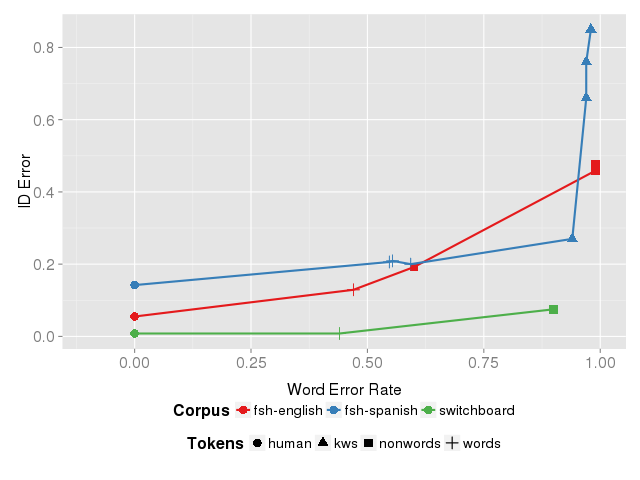
\includegraphics[width=0.75\textwidth]{graphs/wer-err.png}
\caption[Effects of ASR errors on Topic ID]{\label{baseline1}Effect of ASR errors on topic classification of informal speech.}
\end{figure}

If we collect reported classification error rates on available informal speech corpora (LDC's Fisher English and Spanish, Switchboard), we can plot them against the reported (or estimated\footnote{We have included only word-based systems in this graph, for which we can compute WER. For word-spotting systems, we estimate WER from keyword detections, treating all other words as out-of-vocabulary.}) WER (cf. Figure~\ref{baseline1}).  Our own experiments on the Fisher Spanish 25-topic task are the most comprehensive, in terms of variety of error conditions and illustrate that the topic information necessary for this particular task resides in at most 10-20\% of the word tokens.

%In short, subword, out-of-language, and unsupervised techniques exhibit higher ID error rates than word-based ASR, in most cases by an order of magnitude.   A summary of historical Topic ID error results, for the available informal speech corpora, ordered by WER where available, is given in Figure~\ref{baseline1}.    The two noticeable outliers in the Low Resource category are an English phonetic ASR system, which, as stated earlier still doubles the error rate of the comparable word-based system, and the Spanish keyword spotter detailed in \cite{wintrode2014}.  We plot the ID error rates on a log scale so as to emphasize order of magnitude changes.


\subsection{Within Document Locality}

Much of the literature regarding topic classification of speech focuses on corpora where topic labels are applied at the whole-document level. However, it is realistic to suppose that during an actual conversation, lecture, or other informal spoken document, participants may speak on multiple subjects at various points within the document.  Separating a document into coherent topical regions, \textit{topic segmentation} can be considered a task unto itself or useful for downstream retrieval tasks.

Early on in the information retrieval literature, it was recognized that the ``subtopic structuring" of documents could be used to improved full-document retrieval \cite{hearst1993subtopic}.  Hearst's TextTiling algorithm \cite{hearst1997}, used in the aforementioned document retrieval experiments, is the most widely sited text segmentation algorithm in the literature and relies exclusively on bag-of-words ``lexical co-occurrence patterns" roughly at the paragraph level.  We would argue that her results indicate that information relevant to a particular query is often localized in sub-sections of the document.

A number and variety of algorithms have sought to improve on the straightforward sliding-window approach of the TextTiling algorithm.  Reynar's Ph.D.\ thesis refers to the notion of a ``topic shift" in developing his segmentation algorithm \cite{reynar1999}.  Choi's C99 algorithm \cite{choi2000} improves on TextTiling in terms of speed and accuracy.   

In terms of segmentation, Bayesian or latent topic models provide a simple framework for expressing this notion of `subtopic-structuring'.  In a Bayesian sense, a topic is defined simply as a distribution over the corpus vocabulary \cite{wallach2006}.  Given this definition, we can define a document as generated by a weighted mixture of topic distributions.  For segmentation, the latent topic distributions of a document vary from region to region within that document.  We will discuss latent topic models and their relationship to language models in depth in subsequent sections, but a number of improved topic segmentation models have been developed using Bayesian topic modeling technique.  

The current state of the art techniques, Du et al.'s Structured Topic Models \cite{du2013topic} and Ngyuen et al.'s SITS (Speaker Identity for Topic Segmentation) model \cite{nguyen2012sits} have also been evaluated on informal meeting speech.  The ICSI meeting corpus \cite{janin2003icsi} has been annotated to include topic segments.  The only other corpus of informal speech, to our knowledge, annotated at this level of granularity is the CallHome Spanish corpus, which was annotated to study discourse structure \cite{Ries2000}.  However, most corpora are not annotated to this level, so segmentation effects can only be evaluated implicitly.

% locality and classification.
Given the lack of segment-level labels, there is some work being done to consider the effect of topic locality on the classification task. In our own work, we applied the assumption underlying in Hearst's IR work - that not all document segments need to be relevant to the query - to the classification task.   We focused on an aspect of  LDC's informal corpora, whereby participants begin discussing the prompted topic, then drift off-topic as the conversation progresses.  We found that by modeling this \textit{topic drift} explicitly in a bag-of-words framework, we could reduce the ID error rate by 23-47\% \cite{wintrode2013}.  By contrast, in the Reuters text categorization corpus, we found no evidence of topic drift, at least as far as impacted ID error.  We will consider these results in more detail in Chapter 3.

Our assumption that the labeled topic in a supervised setting is most prominent at the \textit{beginning} of a spoken document need not be true, and is almost certainly too restrictive in general.   Recent work on a ``theme identification" task for call centers by Morchid et al.\ considers a location-dependent model for classification \cite{morchid2013theme}.  Here, location is discretized to one of four quantiles of the spoken document and improves classification accuracy by 7\% over a comparable bag-of-words system.  In this case, no restriction is placed on which quantile is most relevant to the task.

% what about the paper in my backpack, that sort of fits here....

% is this conclusion still valid
We would draw two main conclusions from the body of work on topic characterization (to include both classification and segmentation) of speech.  First, as we have mentioned is the robustness to ASR errors of topic information in terms of the `subject of discourse'.  Second is the weakness of typical bags-of-words models, given the loss of information about word locations. We are certainly not the first to point out the limitations of the bag-of-words assumptions, but we would simply highlight the role of location or proximity in word usage.  As we consider other formal models of language for speech recognition and retrieval we will again notice how the locality of word usage must be taken into consideration.

%Before moving on to considering the role of topicality in the \textbf{Tokenization} and \textbf{Retrieval} stages of the speech retrieval pipeline, we would summarize the effect of locality on direct classification \textbf{Models} as reflecting a major potential weakness of bag-of-words models.  The within-document topic dynamics noted in the segmentation literature, the location-aware classifiers (cf. \cite{wintrode2013}, \cite{morchid2013theme}), and Hearst's aforementioned IR work all highlight the weak assumptions of the bag-of-words representation of documents.  We are certainly not the first to point this out, but it is worth mentioning that topic locality results discussed here suggest we definitely look past bag-of-words (if I had said beyond, there would be way too many papers to cite).


%\section{Language Models}
%
%Whereas a statistical topic classifier aims to estimate the probable topic context of a document from its words, language models aim to estimate the probabilities of word sequences, usually given some immediate context.  In the abstract, language models aim to give an estimate for the quantity $P(W)$ where $W$ is a sequence of words $\{w_1,w_2,\ldots w_n\}$.  In the context of \textbf{tokenization}, $P(W)$ arises in the standard noisy channel formulation of speech recognition for tokenizing acoustic observations $O$:
%\begin{equation}
%\hat{W} = \argmax_{W} P(O|W)\cdot P(W)
%\end{equation}
%
%Without any assumptions, this can be rewritten as: 
%\begin{equation}
%P(W) = P(w_1) \cdot P(w_2|w_1)\cdot P(w_3|w_2 w_1) \ldots P(w_n|w_{n-1}\ldots w_1)
%\end{equation}
%
%By replacing the actual history, $h_i=w_{i-1},\ldots w_1$ with one of $M$ equivalence classes over histories $\Phi(h_i)$ we arrive at a general formulation of language modeling \cite{Jelinek1997}.  N-gram language models are one choice for the set of equivalence classes.  In a Bayesian topic model such as Latent Dirichlet Allocation (LDA) \cite{blei2003latent}, the topic state (which is of course un-observed) of $w_i$ provides the equivalence class.  We apply this definition to our problem by claiming that  the $\Phi(h_i)$ for a particular word is affected by the topic of the document localized to where $w_i$ occurs.
%
%\begin{equation}
%P(w_i|h_i) \sim P(w_i | \Phi(h_i))
%\end{equation} 


\section{Speech Recognition}
\label{sec:bkgASR}
%Locality aware language models came first (ish)
In the context of speech recognition, a number of efforts have been made to augment traditional N-gram language models with topic information.  While there is a broader literature focused on the general problem on modeling word sequences, such as incorporating syntax or approaches to N-gram frequency estimation, we highlight efforts on topic and locality in particular.

Two flavors of models have been examined, each focusing on a different aspect of topicality.  Cache-based language models (also referred to as adaptive or trigger models) attempt to exploit the `burstiness' property of language, that is, words are more likely to repeat within the same document.  Topic mixture models look to exploit the different word co-occurrence patterns that occur when different topics are discussed within a document.  These two areas correspond to our definitions of local and broad topic context, respectively. 

Cache-based language models assume that the probability of a word or N-gram in a given word sequence $W$ is influenced both by the global frequency of that word or N-gram as well as the frequency within the current document or preceding $K$ words.  The intuition behind this assumption is that most words are rare at a corpus level, but when they occur, they occur in bursts.   Because of this, a local frequency estimate, such as from a $K$ word `cache' of recently observed words, may be more reliable than the global frequency.  Such a cache or adaptive approach has the advantage of being straightforward to implement.   Jelinek \cite{jelinek1991} and Kuhn \cite{kuhn1990} both find benefits to using these types of models for speech recognition.  Rosenfeld also examined adaptive models within a maximum entropy framework, focusing on what he referred to as `trigger pairs', and also realizing significant gains in WER\cite{rosenfeld1994}.  More recently, Singh-Miller and Collins adapted Rosenfeld's work to improve discriminative language models for N-best and lattice rescoring\cite{singh2007trigger}. 
% church paper?

Adaptive or cache-based language models leverage what is referred to elsewhere as the contagion property of words.   Backoff and smoothing techniques for traditional N-gram models have also aimed to model this property, in order to better account for observed word frequency distributions.  Arguably the most effective N-gram language model technique, Modified Kneser-Ney smoothing \cite{chen1996empirical}, captures this property of language and has proved highly effective for speech recognition.   Beeferman et al., building on Rosenfeld's trigger models developed a model based on expontial families to model the distance between trigger pairs based on the empirical measurements of the strength of this contagion property\cite{beeferman1997}.  Beeferman's model was initially applied to text segmentation\cite{beeferman1999} rather than speech recognition.   We will discuss the contagion property with respect to language models and its relation to topicality in more detail in the last section of this chapter. 

While cache-based or trigger models focus on information within the current document, topic-based mixture models aim to incorporate information based on word usage patterns across documents.   The basic idea is to identify in some way the topic or topics in the document to be processed and then to use topic-specific language models in place of or interpolated with  a base language model to do the particular computation (decoding, re-scoring, or simple likelihood computation).  In some respects, using topic information in this way can considered a form of domain adaptation.

Techniques that attempt to incorporate topics in this manner must first construct a set of topic-dependent language models on training data. This could be done by explicit labels, in supervised setting, or by learning clusters or latent topic models on the training data.   Work in 1999 by Florian and Yarwosky \cite{florian1999} and Khudanpur and Wu \cite{khudanpur1999} aim to create topic-dependent N-gram models using a clustering approach.  In their work, explicit topic labels were assigned to training to documents via vector-space clustering methods, and then counts taken from the labeled partitions.   For speech recognition, first pass output must be used to decide which topic model or models will be interpolated with the global N-gram model.   This approach was shown to decrease WER by up to 1\% absolute.

Other approaches, using LDA\cite{blei2003latent}, PLSA \cite{hofmann2001}, or similar latent variable mixture models have been proposed similar to the works by Florian and Khudanpur.  However, instead of vector-space clustering, topic inference is done within a probabilistic framework, either at training or decoding time.  Both Heidel \cite{heidel2007language} and Hsu \cite{hsu2006} use latent topic mixture models to re-score N-best hypotheses using a mixture of topic-dependent and topic-independent N-gram language models based on the inferred topic distribution of the test document.  In Hsu's work, however, a hard clustering of documents, rather than latent states, is used when training topic-dependent N-gram models.  The work by Hsu resulted in a 2.4\% reduction in WER on the MIT Lectures data set.  Similar (though smaller) gains were observed by Liu et al.\ on Mandarin broadcast conversation \cite{liu2008} and by Huang et al.\ on the AMI meeting corpus \cite{huang2008unsupervised}.
% heidel  - a hard clustering is 

% \cite{naptali2012}  - 0.5\% wer reduction
Almost exclusively, the works cited above focus only on \textit{re-scoring} recognizer output.  However, the lattice of possible word sequences (and by implication any N-best list) are generated and pruned using the original acoustic and language models.  If a word sequence that is more likely under the topic models gets pruned before re-scoring, having a good topic-dependent model does not help.  

% dan asked for perplexity numbers... make sure they're there
In the context of latent topic models, we can explicitly define a topic-dependent unigram language model for any given document $d$, once we have inferred, through any technique, the mixture of topics for that document, $\theta^{(d)}$.   For a latent topic model with $T$ topics, $\theta^{(d)}$ is a $T$-dimensional vector where each element $i$ is the fraction of $d$ that can be attributed to topic $i$.  Practically, $\theta^{(d)}$ acts a mixture weight so that the unigram language model associated with $d$ is given as:

\begin{equation}
P(w) = \sum_{i=1}^T\theta^{(d)}_i \cdot P(w|topic_i)
\end{equation}

In recent work, we found that interpolating these document-specific unigram models with the base N-gram model and using this topic-biased model for decoding did indeed have a significant effect on the pruning of keywords.   We took four languages from the first and second evaluation periods of the IARPA Babel program \cite{babel} (Tagalog, Vietnamese, Zulu, Tamil) and learned an LDA topic model with 100 topics from the training transcripts.  We used  lattice soft counts from the first pass recognition output in a manner similar to \cite{liu2008} to infer the topic proportions $\theta^{(d)}$ of each document.  From this we could construct topic-biased unigram models for each document which we applied during a second decoding pass.

We verified the impact of topic information on lattice pruning by looking at lattice recall of the Babel evaluation keyword lists (roughly 2-5K words or phrases per language).  Table~\ref{latticeRecall} shows the impact of applying topical unigrams at decoding time, versus the baseline output, measured in terms of the proportion of keyword hits that could be found somewhere in the output lattices.  By merely adding topic-dependent unigrams to the base language model, we were able to preserve 2-5\% of keyword hits from pruning\cite{wintrode2014slta}.

\begin{table}[ht]
\centering
   \begin{tabular}{lcc}
   \textbf{Language} & \textbf{Baseline / Re-score}& \textbf{Re-decode} \\ \midrule
        Tagalog &  0.778 & \textbf{0.792}\\
        Vietnamese & 0.555 & \textbf{0.567}\\
        Zulu &  0.718 & \textbf{0.739}\\
        Tamil &  0.573 & \textbf{0.622}\\ \bottomrule
	\end{tabular}
      \caption[Keyword recall obtained re-decoding with topic-augmented models]{Keyword Recall obtained re-decoding with topic-augmented models.\label{latticeRecall}}
\end{table}

% TRANSITION to RETRIEVAL
        
%The largest difference between the two systems is the lattice recall of the words in the query set.  A second observation is that one need not improve WER to improve search performance.   While these are preliminary results, they seem to indicate that earlier application of topic-dependent language models in the decoding process would benefit the speech retrieval process.  

\section{Retrieval}

Language models have applications not just for decoding, but also during retrieval of documents.  Language model-based retrieval is major area in the information retrieval (IR) community, staring with the work in the late 90's by Ponte and Croft \cite{ponte1998}.  Incorporating topicality into the retrieval language models, as with Heart's use of locality, has improved retrieval performance.  

In many text retrieval tasks, queries are often tens or hundreds of words in length rather than short spoken phrases.  The likelihood of the query word sequence is then evaluated under a document-specific language model.   Similar to the manner in which we computed a topic-dependent model from the per-document topic proportions $\theta_d$, multiple efforts in the IR community have used LDA or similar techniques to compute a topic-dependent document model  (cf. \cite{wei2006lda}, \cite{chen2009}, \cite{liu2004cluster}).  In these efforts, the topic model information was helpful in boosting retrieval performance above the baseline vector space or N-gram models.


As previously discussed, topicality also arises in the \textbf{burstiness} property of language.   Church and Gale examine this property in great depth in their studies of document frequency \cite{church1999}, Poisson mixtures, \cite{church1995poisson}, and word adaptation \cite{church2000}.   Looking at content words in the Brown corpus, they illustrate how content words tend to not be evenly distributed across a corpus (as a Poisson generative assumption would predict), but instead occur in bursts in a small number of documents or topics (genres) \cite{church1995poisson}.  

\begin{figure}[t]
\begin{center}
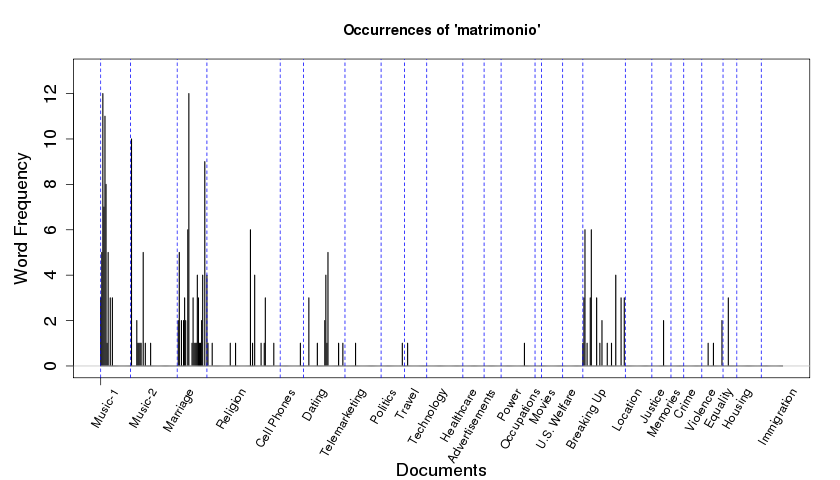
\includegraphics[width=0.7\textwidth]{graphs/freq-matrimonio.png}
\caption[Word frequencies of \textit{matrimonio} by topic]{Word frequencies of \textit{matrimonio} (marriage) in documents grouped together by topic.\label{spanishBursts}}
\end{center}
\end{figure}

 %ganguly2011utilizing
As an example of this phenomenon, we can visualize these bursts on LDC's Fisher Spanish corpus (as Church and Gale did for the Brown corpus) by plotting the frequency of content words in each document, grouping documents with the same topic label adjacent to one another.  Documents are given as points on the horizontal axis and dashed blue lines indicate topic boundaries.  We can compare the plot for \textit{matrimonio} (marriage, cf. Figure~\ref{spanishBursts}) with the same plot for a more common word \textit{juntos} (together, cf. Figure~\ref{spanishBurst2}).  


\begin{figure}[t]
\begin{center}
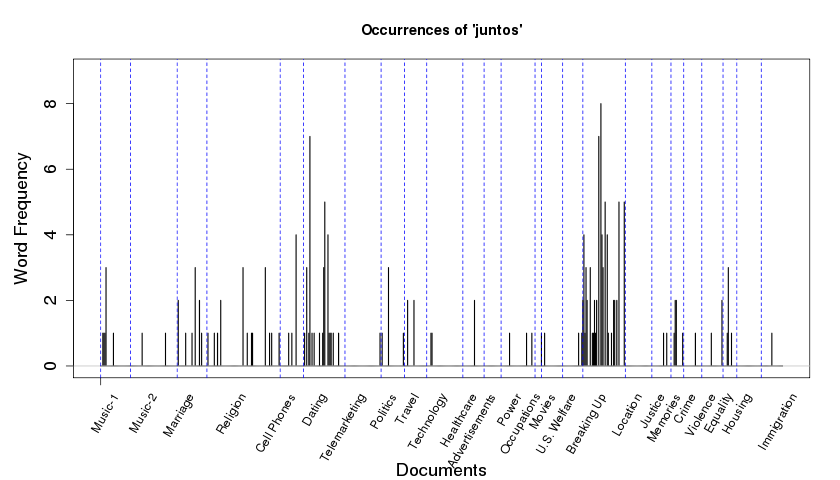
\includegraphics[width=0.7\textwidth]{graphs/freq-juntos.png}
\caption[Word frequencies of \textit{juntos} by topic]{Word frequencies of \textit{juntos} (together) in documents grouped together by topic.\label{spanishBurst2}}
\end{center}
\end{figure}

While \textit{juntos} is commonly used in contexts unrelated to human relationships, there are noticeable bursts in the \textit{Dating} and \textit{Breaking Up} topics.  Taking the $\chi^2$ statistic, used for selecting strongly correlated features for text classification (cf. \cite{yang1997}), we obtain scores of 46.2 and 323.4 for \textit{juntos} co-occurring with those two topics, respectively.  For 25 topics, a $\chi^2$ of greater than 44.3 indicates a 99\% confidence of a correlation between the frequency of \textit{juntos} and a given topic label.  Conversely, the scores for \textit{juntos} and the other 23 topics are less than 11.5, which is the 1\% confidence level, as a score of 0 indicates no correlation.  In these cases, we are comfortable relating the burstiness in particular documents to the underlying topic.

By contrast, the function words \textit{el} and \textit{como} - `the' and `how' respectively - while quite variable in the frequency with which they occur in particular documents, are not as clearly correlated with particular topics (cf. Figures~\ref{freqEl},\ref{freqComo}).  The highest correlated topic for \textit{como} according to the $\chi^2$ metric is \textit{Memories} with a score of 21.4, which is outside the confidence interval.  However, the word \textit{el}, according to the $\chi^2$ metric, is correlated with the \textit{Power} topic with a score of 122.0.   The word \textit{el} is clearly repeated quite frequently in all documents, but it seems hard to argue that this is because it is closely related to the subject matter.

\begin{figure}
\begin{center}
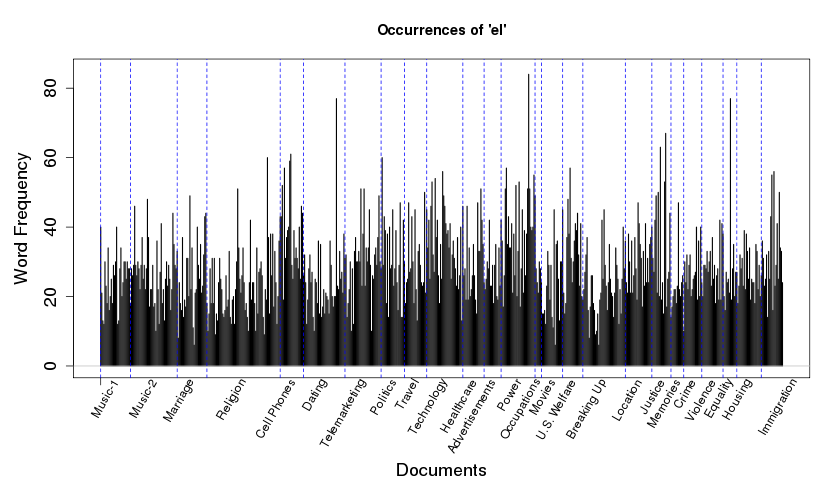
\includegraphics[width=0.7\textwidth]{graphs/freq-el.png}
\caption[Word frequencies of \textit{el} by topic]{Word frequencies of \textit{el} (the) in documents grouped together by topic.\label{freqEl}}
\end{center}
\end{figure}

\begin{figure}
\begin{center}
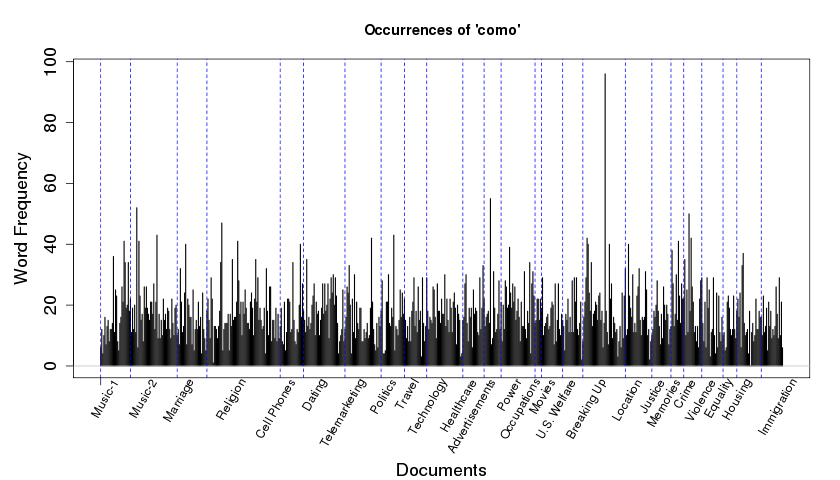
\includegraphics[width=0.7\textwidth]{graphs/freq-como.png}
\caption[Word frequencies of \textit{como} by topic]{Word frequencies of \textit{como} (how) in documents grouped together by topic.\label{freqComo}}
\end{center}
\end{figure}

We will look at the application of both burstiness (or local context) and topic information (broad context) to the retrieval task in Chapter~\ref{sec:topicLMsRetrieval}.  The burstiness property (or contagion) can account for the power law distribution of word frequencies in a corpus.  With this in mind, we conclude this discussion of topics within research areas surrounding speech recognition and retrieval by looking at how topics arise in different formal frameworks for statistical language modeling.  


\section{Generative Models of Language}
We have heretofore discussed language models and latent topic models (LDA) somewhat  interchangeably.  In this section we want to sketch the relationship between N-gram language models and latent topic models, focusing on the burstiness or contagion property.   Given the properties of these models, we would then propose our own building on the strengths and weaknesses for our stated task.

\subsection{Urn Models}

There is a family of models, mostly attributed to George Pólya, which can be used to model the burstiness phenomena in language.   In the multivariate formulation, we consider an urn filled with balls of $V$ different colors, initially containing $x_i$ balls of color $i$.  At each point in time one is drawn, its color noted.  This ball is then replaced along with an additional $c_i$ balls of the same color.  This $c_i$ is often referred to as the contagion parameter.  

Thus `burstiness' is modeled as a rich-get-richer scenario.  If we use words tokens instead of balls and word types in place of colors, we have a simple generative model for corpora.  If we have initial counts $x_i$ and let $n_i$ be the number of additional words of type $i$ that have been drawn, the probability of a particular word at this time in the generative process is given as:
\begin{equation}
P(color_i) = \frac{x_i + n_i\cdot c_i}{\sum_{j=1}^V \left (x_j + n_j \cdot c_j\right)}
\label{urn}
\end{equation}

One of the properties of Pólya urn models is \textit{exchangeabilty}: the probability of an $n$-length sequence of draws depends only on the number of balls drawn of each color, not on the order in which they are drawn.  This property is also evident in bag-of-word models, which represent only counts of words and not their order.

Pólya urn models arise in the related distributions in latent topic modeling: multinomials (the topics) and the Dirichlet (the prior on the multinomials).  At the limit, the proportion of balls in the urn scheme is distributed as a Dirichlet with parameters $(c_1,\ldots,c_V)$ identical to the contagion parameters on the urn\cite{blackwell1973}.  Multiple authors also note that the Dirichlet-Multinomial is a Pólya distribution, arising from such an urn scheme (cf. \cite{minka2000estimating}, \cite{madsen2005modeling}, \cite{mimno2011optimizing}).  In a Bayesian setting such as Latent Dirichlet Allocation (LDA), the hyperparameter $\beta$ for the Dirichlet prior of the multinomial topic word distribution is viewed as a smoothing constant or concentration parameter\cite{wallach2006}.  In the Bayesian sense this is intuitive, given a $V$-dimensional Dirichlet acts as a distribution over $V-$dimensional multinomials.  But in terms of an urn model, $\beta$ is simply a uniform contagion parameter.

%Polya urn models.  Property of these models is the ``exchangeability".  The contagion parameter gives the desired power law behavior.

%Minka, Mimno, Madsen -  Indeed we can conceptualize a Gibbs Sampling procedure as simulating draws from Polya's urn, letting the contagion parameter generate the appropriate power law distribution. 

We can characterize the relationship between latent topic models like LDA and these Dirichlet-Multinomial urn models as many to one.  The LDA generative model holds that a document is generated from a weighted mixture of $K$ topics (i.e. Dirichlet-Multinomial unigram models).  In contrast, a cache or adaptive language model is a single constrained urn model, where the initial contents of the urn are given by the base N-gram language model, and the contagion parameters are captured by the interpolation weight.

%Contrast  with cache or adaptive language models, in which the corpus is generated from a single such model over N-grams.
%
%Estimation 
%1. Describe an existing corpus - parameter estimation 
%
%Inference
%2a. Predict words - n-gram models in speech recognition, term detection
%2b. Predict latent variables (i.e. Topics)
%
%In terms of latent variables, 2b is very similar to 1. 2a 
%ngram models - multinomial models  - even in backoff/smoothing, if necessary can enumerate $\theta$
%multinomial -> ngram -> 
%add latent state to get 
%poisson mixture -> misture of multinomials


\subsection{Dirichlet Processes}

Urn models can also be thought as arising out of a class of models called Dirichlet processes.   Dirichlet processes are thought of as ``distributions of distributions."\cite{teh2010dirichlet}   In particular, Pittman-Yor processes, which are a particular family of Dirichlet processes, have been shown to relate to both N-gram language models and to Dirichlet-Multinomial mixtures (i.e. LDA).  % more detail?


\begin{figure}[t]
\centering
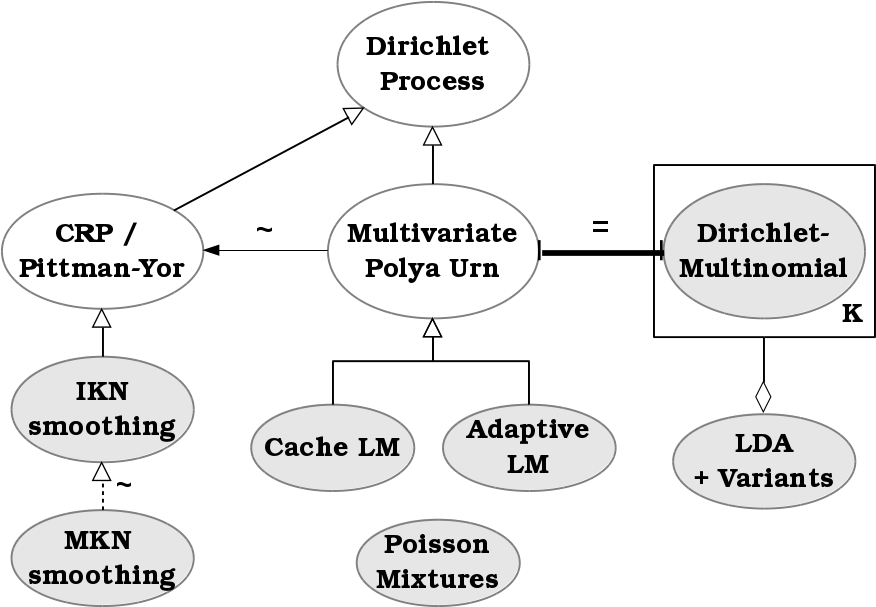
\includegraphics[width=0.8\textwidth]{lms.png}
\caption[Models of word generation]{Relationships between various models of word generation.\label{topicLMS}}
\end{figure}


Both Goldwater et al.\cite{goldwater2011} and Teh \cite{teh2006} demonstrate the equivalence between Interpolated Kneser-Ney (IKN) language models and what Teh calls ``hierarchical Pittman-Yor" language models and what Goldwater et al.\ refer to as a ``two stage" Pittman-Yor process.   Teh also argues that Modified Kneser-Ney (MKN) is an approximation to this hierarchical Bayesian non-parametric model.

%3. PY/CRP/polya urn/ stick breaking = DCM = IKN ~ MKN
% wang & blei 2012
% 

A stylized UML diagram of the relationship between various language and topic models, based on the previous discussion and showing direct generalization where possible, is presented in Figure~\ref{topicLMS}.  This is meant to be illustrative, not authoritative or exhaustive.

One final note contrasting MKN or IKN with a cache or adaptive language model, which is directly related to our work in this area.   At recognition time, with a typical N-gram language model, the urn is fixed, so to speak.  A cache model on the other hand allows the generative process to continue and recognition to benefit from the topic information in the unseen document (at a cost).  

In Dirichlet-Multinomial mixture models such as LDA and variants or any the latent variable models such as Du et al.'s Structured Topic Models for example, one of the principle modeling challenges is estimating the unobserved (latent) parameters from the observed data (word sequences).  In the literature, this task is referred to as \textit{approximate posterior inference}, and as topic information is often expressed as a latent property of the data we will introduce the most common techniques here.  We will refer back to these techniques in Chapter 5 when we develop our own cache-augmented latent topic model.

\section{Posterior Inference}
\label{sec:postInf}
We now describe the most common posterior inference techniques.  In the context of speech retrieval we will distinguish \textit{estimation}, whereby we learn model parameters on some training corpus, and \textit{inference}, where we obtain the latent variable state on unseen or held-out data (i.e. the ASR development or test set).  Nonetheless, both steps are examples of approximate posterior inference, in which the latent variable properties are learned from observed data.

Posterior inference techniques typically applied to graphical models can be categorized as Variational Bayes (VB) or Markov Chain Monte Carlo (MCMC) techniques.  Variational Bayes techniques perform optimization on a distribution similar to but simpler than the true posterior distribution, typically via the Expectation Maximization (EM) algorithm.  MCMC techniques estimate the posterior distribution by integrating sampled values from a Markov chain that converges to the desired distribution.

Blei and Jordan, in their original derivation of LDA\cite{blei2003latent}, presented a Variational Bayes method for estimating the LDA parameters.  This is built off of Jordan's early work where he introduces variational methods that leverage Jensen’s inequality to bound the log likelihood\cite{jordan1999}.  In their original paper, Blei and Jordan refer to the topic distributions with the variable $\beta$, and the variational approximation as $\phi$\footnote{Except for here, will use $\phi$ to refer to the original topic distributions, to be consistent with the nomenclature of Stevyvers et al.\cite{steyvers2007} and related work}.  The variational approximation to the topic mixtures $\theta$ is given as $\gamma$.  Blei and Jordan show that the Kullback-Leibler divergence between the true posterior distribution (conditioned on the true parameters $\beta,\theta$) and the variational distribution $q(\theta,z|\gamma,\phi)$ can indeed be optimized using the EM algorithm.  
\begin{equation}
(\gamma^*, \phi^*) = \underset{(\gamma,\phi)}{\arg \min}\,\text{D}\left[q(\theta,z|\gamma,\phi)\|p(\theta,z|w,\alpha,\beta)\right]
\end{equation}

\nocite{hoffman2010online} 

The variational approach necessitates finding some appropriate $q$ that is tractable for optimization techniques.  The second approach to posterior inference is a set of sampling techniques referred to as Markov Chain Monte Carlo.  MCMC sampling was first introduced by Metropolis et al.\cite{metropolis1953equation} in their work on modeling behavior of atomic particles and generalized in a statistical framework by Hastings in 1970 \cite{hastings1970monte}.

The basic idea is arrived at by combining the definition of the expected value of a continuous random variable and Monte Carlo approximations of integrals.  The expected value $E[f(X)]$ is given by the integral:
\begin{equation}
E\left[f(X)\right] =\int{f(X)\cdot P(X)\,dX} \label{eqn5:expectedValue}
\end{equation}
\noindent The intuition behind MCMC is to apply Monte Carlo methods for numerically approximating the expected value of $X$.

In the specific case of approximate inference, the $X$ we are interested in is just the parameter values given the observed data $W$ (for simplicity, we denote all of our latent parameters $(Z,K,\Theta,\Phi) = X$:
\begin{equation}
E\left[X|W;\alpha,\beta,\nu\right] =\int{X\cdot P(X|W;\alpha,\beta,\nu)\,dX} \label{eqn5:integral}
\end{equation}

\noindent If one could sample from the posterior distribution $P(X|W)$, then one can numerically approximate the interval in Equation~\ref{eqn5:integral} and obtain an estimate of the true value.  The Markov Chain part of MCMC requires one to produce a Markov chain such that as the sampling procedure progresses, the sample approaches (in the limit) a random sample from $P(X|W)$ \cite{brooks1998markov}.  By extension, averaging samples from the chain gives the desired expected value estimate.

Two related MCMC sampling techniques that produce such a Markov Chain are \textbf{Gibbs Sampling} and the \textbf{Metropolis-Hastings} algorithm.  Gibbs Sampling proceeds by sampling one unobserved variable at a time, conditioned on the observed data \textit{and} the current sampler state for the other unobserved values.   By the sampler state, we mean the currently sampled values temporarily assigned to the unobserved variables.  In our model this would mean sampling each $z_{d,i}$ and then each $k_{d,i}$ given the observed words and current state of the other sampled variables $Z$ and $K$.  The Markov Chain properties of the procedure ensure that as we proceed, the sampled values approach the expected values of the topic and cache states given the observed words.  In layman's terms, the expected value gives us the best approximation for the topic and cache mixture underlying the observed words.

In the general case, assuming a series of latent states $Z=\{z_1,\ldots,z_n\}$ and observations $X=\{x_1,\ldots,x_m\}$, Gibbs sampling proceeds as follows.   Assign some initial values to the states $Z$.  Then, iteratively, for each $z_i$, sample a new value for $z_i$ according to the distribution $P(z_i|Z_{-i},X)$.  As elsewhere, the subscript $-i$ indicates that the sequence does not contain the $i^{th}$ item. 

Gibbs Sampling can be shown to be a specific case of the Metropolis-Hastings algorithm (see \cite{brooks1998markov} for a full overview of the various MCMC techniques).   Metropolis-Hastings constructs the Markov Chain of samples for the unobserved variables by means of \textit{proposal distribution} (also called a \textit{jumping distribution}).  The proposal distribution is used to suggest samples, given the current sampling state.  Any function $f(Z,X)$ which is proportional to the posterior distribution $P(Z|X)$ we are trying to approximate is used to accept or reject proposed samples, making Metropolis-Hastings a form of \textit{generalized rejection sampling}.  

If the current sampling state is $Z^t$ and a new value $z^\prime$ is proposed for $z_i$, then with Metropolis-Hastings, the acceptance probability $\alpha$ of that particular sample is calculated as:
\begin{equation}
\alpha=\min\left\{1,\frac{f(z^\prime,Z^t_{-i},X)}{f(Z^t,X)}\right\}
\end{equation}
The new sampling value is assigned to the sampling state for $z_i$ with probability $\alpha$.

In the Gibbs Sampling instance of Metropolis-Hastings, the proposal distribution is simply the distribution $P(z_i|Z_{-i},X)$ and samples are always accepted.  In practice, this need not be the case.  A \textit{burn-in} period may be used, where samples are dropped from the first $N$ iterations, so as to allow the Markov process to move away from the initial conditions to a steady state.   Another alternative is to use \textit{thinning} where only a proportion of samples are kept.  The effectiveness of either technique is best judged empirically.   % (practically, this need not be the case).

\nocite{steyvers2007}
\nocite{yao2009efficient}

\section{Summary}
% final transition
We have aimed to highlight both the multiple aspects of topicality in language, the theoretical frameworks within which they live and by which they are evaluated, as well as the their successful application to various areas of speech recognition and retrieval.  Given the positive impact of topic information in its various forms discussed in this chapter, we believe it worthwhile to examine this in more depth.


 % in subsequent chapters we aim examine and model local and broad topic contexts explicity.  Jointly leverage these aspects of languagee
